\def\radA{1cm}
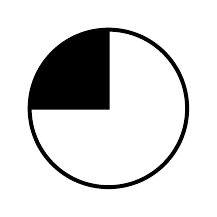
\begin{tikzpicture}[baseline = (current bounding box.west)]


\node[draw, circle, minimum size=2*\radA, inner sep=0pt, line width=0.5mm, outer sep=0] (circ) at (0,0) {};

%\node[anchor=north, inner sep=2pt, rotate=0] (8cm.label) at ($(circ.center)!0.5!(180:\radA)$) {$ \text{5in}$};

%\node[anchor=south east, inner sep=2pt, rotate=0] (90.label) at ($(circ.center)+(135:\radA)$) {$ 90 \degree $};

\filldraw[fill=\figurefill, line width=0.3mm]  (90:\radA) arc (90:180:\radA) -- (circ.center) -- cycle;

\end{tikzpicture} 
